\chapter{Примеры использования алгоритмов}

Рассмотрим задачу автоматического управления полетом самолета. В такой задаче важное место занимает стабилизация летательного аппарата во всех возможных режимах. Следовательно, нужно построить такой регулятор, который бы с помощью постоянных настроек обеспечивал управление подобного рода. Рассмотрим стабилизацию продольного углового движения многорежимного летательного аппарата.\br

Линеаризованная модель задается следующей системой уравнений:

\begin{equation}
\label{eq:6/1}
\left\{ \begin{array}{l}
\dot{\vartheta} = \omega_z\mbox{,} \\
\dot{\omega}_z = -a_{mz}^\alpha\vartheta - a_{mz}^{\omega z}\omega_z + a_{mz}^\alpha\Theta + a_{mz}^\delta\delta\mbox{,} \\
\dot{\Theta} = -a_y^\alpha\vartheta + a_y^\alpha\Theta\mbox{;}
\end{array} \right.
\end{equation}

где $\vartheta$~--- угол тангажа, $\omega_z$~--- угловая скорость тангажа, $\Theta = a-\alpha$~--- угол наклона траектории, $\alpha$~--- угол атаки, $\delta$~--- угол отклонения руля.

Переменными состояния и управления системы \vref{eq:6/1} будут, соответственно

\begin{equation}
\label{eq:6/2}
x(t) = [\vartheta~\omega_z~\Theta]^T,~~~~u(t)=\delta
\end{equation}

Как правило, для непосредственного наблюдения доступны только $\vartheta$ и $\omega_z$, поэтому \ref{eq:6/2} можно переписать как

\begin{equation}
\label{eq:6/3}
x(t) = [\vartheta~\omega_z]^T,~~~~u(t)=\delta
\end{equation}

Предполагаем, что летательный аппарат имеет 9 различных режимов полета с заданными числовыми значениями параметров:

\begin{equation*}
\begin{array}{lr}

%------------------------------------
A_1^0 = \left(\begin{array}{ccc}
0     &     1     &     0 \\
-4    &     1.4   &     4 \\
0.62  &     0     &     -0.62
\end{array}\right)\mbox{,} &
B_1^0 = \left(\begin{array}{c}
0 \\
-7.5 \\
0
\end{array}\right)\mbox{;} \\
%------------------------------------
A_2^0 = \left(\begin{array}{ccc}
0     &     1     &     0 \\
-4.2    &     -1.5   &     4.2 \\
0.77  &     0     &     -0.77
\end{array}\right)\mbox{,} &
B_2^0 = \left(\begin{array}{c}
0 \\
-7.4 \\
0
\end{array}\right)\mbox{;} \\
%------------------------------------
A_3^0 = \left(\begin{array}{ccc}
0     &     1     &     0 \\
-7.1    &     -1.9   &     7.1 \\
1  &     0     &     -1
\end{array}\right)\mbox{,} &
B_3^0 = \left(\begin{array}{c}
0 \\
-12.7 \\
0
\end{array}\right)\mbox{;} \\
%------------------------------------
A_4^0 = \left(\begin{array}{ccc}
0     &     1     &     0 \\
-7.9    &     -1.1   &     7.9 \\
0.56  &     0     &     -0.56
\end{array}\right)\mbox{,} &
B_4^0 = \left(\begin{array}{c}
0 \\
-13.8 \\
0
\end{array}\right)\mbox{;} \\
%------------------------------------
A_5^0 = \left(\begin{array}{ccc}
0     &     1     &     0 \\
-14.5    &     -0.43   &     14.5 \\
0.33  &     0     &     -0.33
\end{array}\right)\mbox{,} &
B_5^0 = \left(\begin{array}{c}
0 \\
-8.6 \\
0
\end{array}\right)\mbox{;} \\
%------------------------------------
A_6^0 = \left(\begin{array}{ccc}
0     &     1     &     0 \\
-18    &     -0.31   &     18 \\
0.34  &     0     &     -0.34
\end{array}\right)\mbox{,} &
B_6^0 = \left(\begin{array}{c}
0 \\
-10 \\
0
\end{array}\right)\mbox{;} \\
%------------------------------------
A_7^0 = \left(\begin{array}{ccc}
0     &     1     &     0 \\
-55    &     -0.66   &     55 \\
0.84  &     0     &     -0.84
\end{array}\right)\mbox{,} &
B_7^0 = \left(\begin{array}{c}
0 \\
-22.5 \\
0
\end{array}\right)\mbox{;} \\
%------------------------------------
A_8^0 = \left(\begin{array}{ccc}
0     &     1     &     0 \\
-78    &     -4.1   &     78 \\
2.8  &     0     &     -2.8
\end{array}\right)\mbox{,} &
B_8^0 = \left(\begin{array}{c}
0 \\
-57 \\
0
\end{array}\right)\mbox{;} \\
%------------------------------------
A_9^0 = \left(\begin{array}{ccc}
0     &     1     &     0 \\
-116    &     -2.36   &     116 \\
2.3  &     0     &     -2.3
\end{array}\right)\mbox{,} &
B_9^0 = \left(\begin{array}{c}
0 \\
-42 \\
0
\end{array}\right)\mbox{;} \\


C_{i0} = \left(\begin{array}{ccc}
1 & 0 & 0 \\
0 & 1 & 0
\end{array}\right)\mbox{,} &
i \in \{1,2,\ldots,N\}\mbox{.}


\end{array}
\end{equation*}

Используя алгоритмы робастной и одновременной стабилизации (\vref{alg:4/3} и \vref{alg:4/2} соответственно) была получена матрица усиления $F = [-11.8~~-0.6]$, стабилизирующая все системы. К сожалению, общую функцию ляпунова удалось построить только для первых 7 систем. Используя итерационный алгоритм, была получена матрица $F = [-21.5~~-1.7]$.

На рисунке показаны переходные процессы для последнего случая:

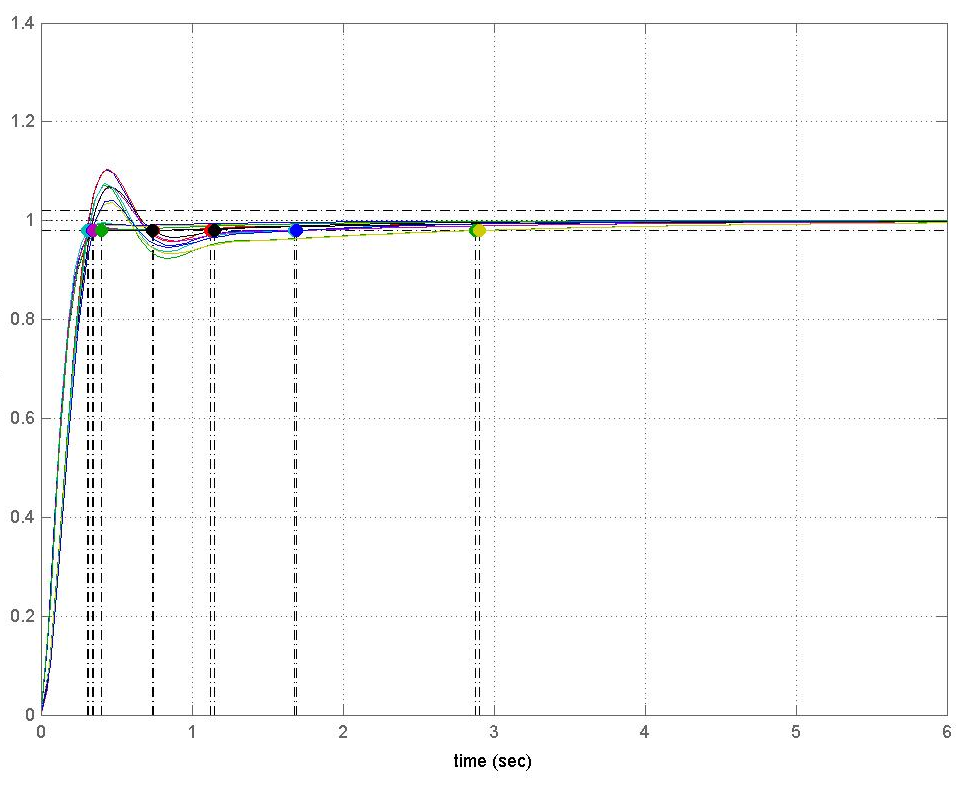
\includegraphics[scale=0.4]{screenshot.png}

Рассмотрим другой пример. Условия те же, но матрицы параметров отличаются.

\begin{equation*}
\begin{array}{lr}


%------------------------------------
A_1^0 = \left(\begin{array}{ccc}
0    &    1    &    0 \\
-14.1996    &    -6.08996    &    14.1996 \\
-2.96787    &    0    &    2.96787
\end{array}\right)\mbox{,} &
B_1^0 = \left(\begin{array}{c}
0 \\
-7.64812 \\
0
\end{array}\right)\mbox{;} \\

%------------------------------------
A_2^0 = \left(\begin{array}{ccc}
0    &    1    &    0 \\
-24.3236    &    -5.01533    &    24.3236 \\
-2.00206    &    0    &    2.00206
\end{array}\right)\mbox{,} &
B_2^0 = \left(\begin{array}{c}
0 \\
-12.3768 \\
0
\end{array}\right)\mbox{;} \\

%------------------------------------
A_3^0 = \left(\begin{array}{ccc}
0    &    1    &    0 \\
-43.0945    &    -5.43643    &    43.0945 \\
-2.72507    &    0    &    2.72507
\end{array}\right)\mbox{,} &
B_3^0 = \left(\begin{array}{c}
0 \\
-20.9305 \\
0
\end{array}\right)\mbox{;} \\

%------------------------------------
A_4^0 = \left(\begin{array}{ccc}
0    &    1    &    0 \\
-61.8141    &    -4.30745    &    61.8141 \\
-2.25735    &    0    &    2.25735
\end{array}\right)\mbox{,} &
B_4^0 = \left(\begin{array}{c}
0 \\
-22.0166 \\
0
\end{array}\right)\mbox{;} \\

%------------------------------------
A_5^0 = \left(\begin{array}{ccc}
0    &    1    &    0 \\
-68.4906    &    -1.5788    &    68.4906 \\
-1.90049    &    0    &    1.90049
\end{array}\right)\mbox{,} &
B_5^0 = \left(\begin{array}{c}
0 \\
-29.1617 \\
0
\end{array}\right)\mbox{;} \\

%------------------------------------
A_6^0 = \left(\begin{array}{ccc}
0    &    1    &    0 \\
-73.3721    &    -1.97372    &    73.3721 \\
-1.24783    &    0    &    1.24783
\end{array}\right)\mbox{,} &
B_6^0 = \left(\begin{array}{c}
0 \\
-36.5696 \\
0
\end{array}\right)\mbox{;} \\

%------------------------------------
A_7^0 = \left(\begin{array}{ccc}
0    &    1    &    0 \\
-85.9945    &    -4.94462    &    85.9945 \\
-1.65782    &    0    &    1.65782
\end{array}\right)\mbox{,} &
B_7^0 = \left(\begin{array}{c}
0 \\
-43.9964 \\
0
\end{array}\right)\mbox{;} \\

%------------------------------------
A_8^0 = \left(\begin{array}{ccc}
0    &    1    &    0 \\
-94.154    &    -8.35004    &    94.154 \\
-1.66214    &    0    &    1.66214
\end{array}\right)\mbox{,} &
B_8^0 = \left(\begin{array}{c}
0 \\
-47.8299 \\
0
\end{array}\right)\mbox{;} \\

%------------------------------------
A_9^0 = \left(\begin{array}{ccc}
0    &    1    &    0 \\
-110.563    &    -6.05252    &    110.563 \\
-0.610667    &    0    &    0.610667
\end{array}\right)\mbox{,} &
B_9^0 = \left(\begin{array}{c}
0 \\
-53.4986 \\
0
\end{array}\right)\mbox{;} \\

C_{i0} = \left(\begin{array}{ccc}
1 & 0 & 0 \\
0 & 1 & 0
\end{array}\right)\mbox{,} &
i \in \{1,2,\ldots,N\}.


\end{array}
\end{equation*}


Матрица усиления по алгоритмам \vref{alg:4/2} и \vref{alg:4/1}: $F = [-9.01~~-1]$. Итерационный алгоритм дал матрицу усиления $F=[-11.4~~-0.9]$.

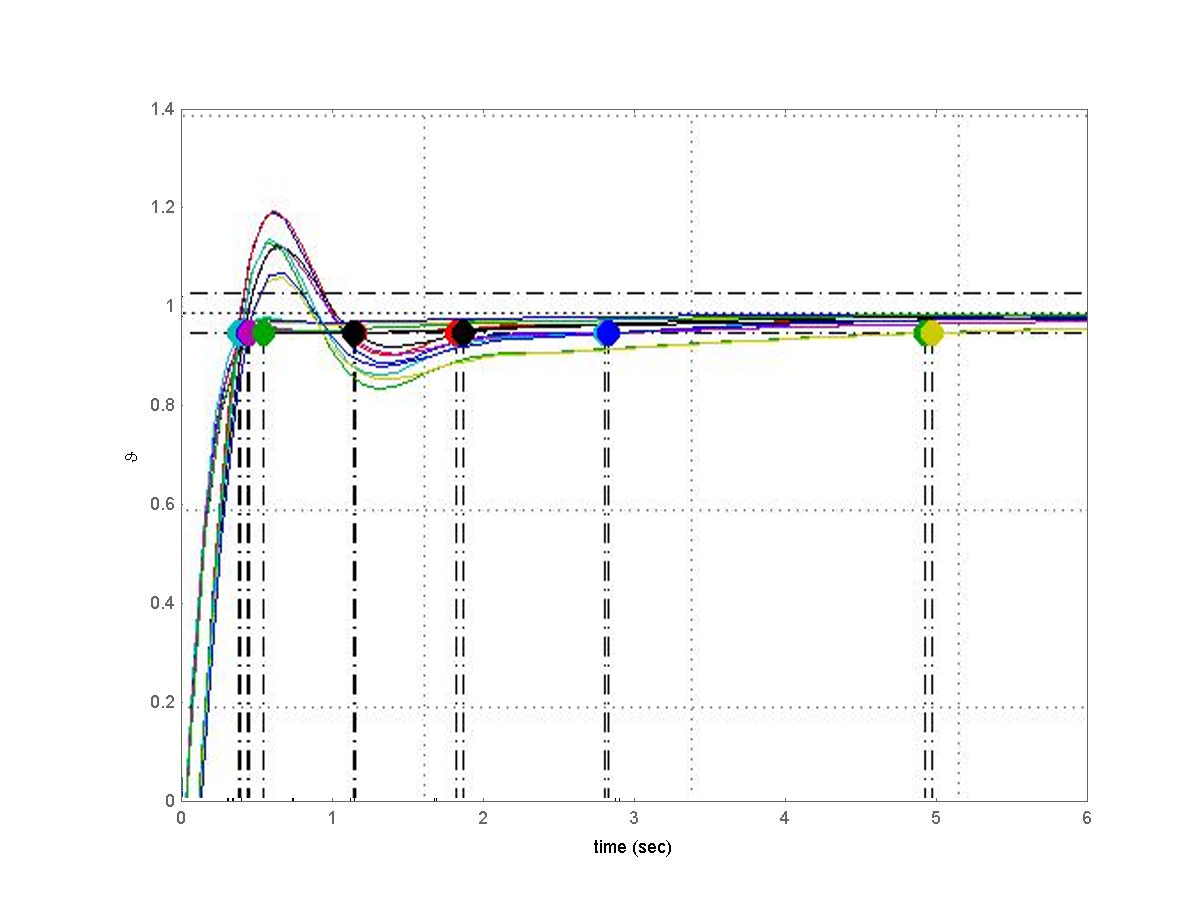
\includegraphics[scale=0.3]{screenshot2.png}

Рассмотрим вырожденный пример, на котором итерационный алгоритм расходится:

\begin{equation*}
\begin{array}{lr}


%------------------------------------
A_1^0 = \left(\begin{array}{ccc}
0    &    1    &    0 \\
12.4502    &    -3.71318    &    12.4502 \\
1.34787    &    0    &    1.34787
\end{array}\right)\mbox{,} &
B_1^0 = \left(\begin{array}{c}
0 \\
-1.06727 \\
0
\end{array}\right)\mbox{;} \\

%------------------------------------
A_2^0 = \left(\begin{array}{ccc}
0    &    1    &    0 \\
24.6718    &    -10.2687    &    24.6718 \\
2.60235    &    0    &    2.60235
\end{array}\right)\mbox{,} &
B_2^0 = \left(\begin{array}{c}
0 \\
-5.75874 \\
0
\end{array}\right)\mbox{;} \\

%------------------------------------
A_3^0 = \left(\begin{array}{ccc}
0    &    1    &    0 \\
34.7688    &    -7.92524    &    34.7688 \\
0.102741    &    0    &    0.102741
\end{array}\right)\mbox{,} &
B_3^0 = \left(\begin{array}{c}
0 \\
-11.3652 \\
0
\end{array}\right)\mbox{;} \\

%------------------------------------
A_4^0 = \left(\begin{array}{ccc}
0    &    1    &    0 \\
37.4861    &    -2.35985    &    37.4861 \\
2.86302    &    0    &    2.86302
\end{array}\right)\mbox{,} &
B_4^0 = \left(\begin{array}{c}
0 \\
-13.5763 \\
0
\end{array}\right)\mbox{;} \\

%------------------------------------
A_5^0 = \left(\begin{array}{ccc}
0    &    1    &    0 \\
39.7132    &    -10.9082    &    39.7132 \\
0.982049    &    0    &    0.982049
\end{array}\right)\mbox{,} &
B_5^0 = \left(\begin{array}{c}
0 \\
-16.5169 \\
0
\end{array}\right)\mbox{;} \\

%------------------------------------
A_6^0 = \left(\begin{array}{ccc}
0    &    1    &    0 \\
58.4972    &    -3.03661    &    58.4972 \\
0.370441    &    0    &    0.370441
\end{array}\right)\mbox{,} &
B_6^0 = \left(\begin{array}{c}
0 \\
-18.5588 \\
0
\end{array}\right)\mbox{;} \\

%------------------------------------
A_7^0 = \left(\begin{array}{ccc}
0    &    1    &    0 \\
66.6071    &    -6.62716    &    66.6071 \\
1.59545    &    0    &    1.59545
\end{array}\right)\mbox{,} &
B_7^0 = \left(\begin{array}{c}
0 \\
-20.3229 \\
0
\end{array}\right)\mbox{;} \\

%------------------------------------
A_8^0 = \left(\begin{array}{ccc}
0    &    1    &    0 \\
70.8975    &    -6.32684    &    70.8975 \\
2.97756    &    0    &    2.97756
\end{array}\right)\mbox{,} &
B_8^0 = \left(\begin{array}{c}
0 \\
-25.7138 \\
0
\end{array}\right)\mbox{;} \\

%------------------------------------
A_9^0 = \left(\begin{array}{ccc}
0    &    1    &    0 \\
87.8503    &    -3.14445    &    87.8503 \\
1.91167    &    0    &    1.91167
\end{array}\right)\mbox{,} &
B_9^0 = \left(\begin{array}{c}
0 \\
-35.2216 \\
0
\end{array}\right)\mbox{;} \\

C_{i0} = \left(\begin{array}{ccc}
1 & 0 & 0 \\
0 & 1 & 0
\end{array}\right)\mbox{,} &
i \in \{1,2,\ldots,N\}.
\end{array}
\end{equation*}

Итерационный алгоритм расходится. Алгоритм \vref{alg:4/2} дал же матрицу усиления $F = [-15.9567~~-1.002]$
